\begin{figure}[htbp]\centering
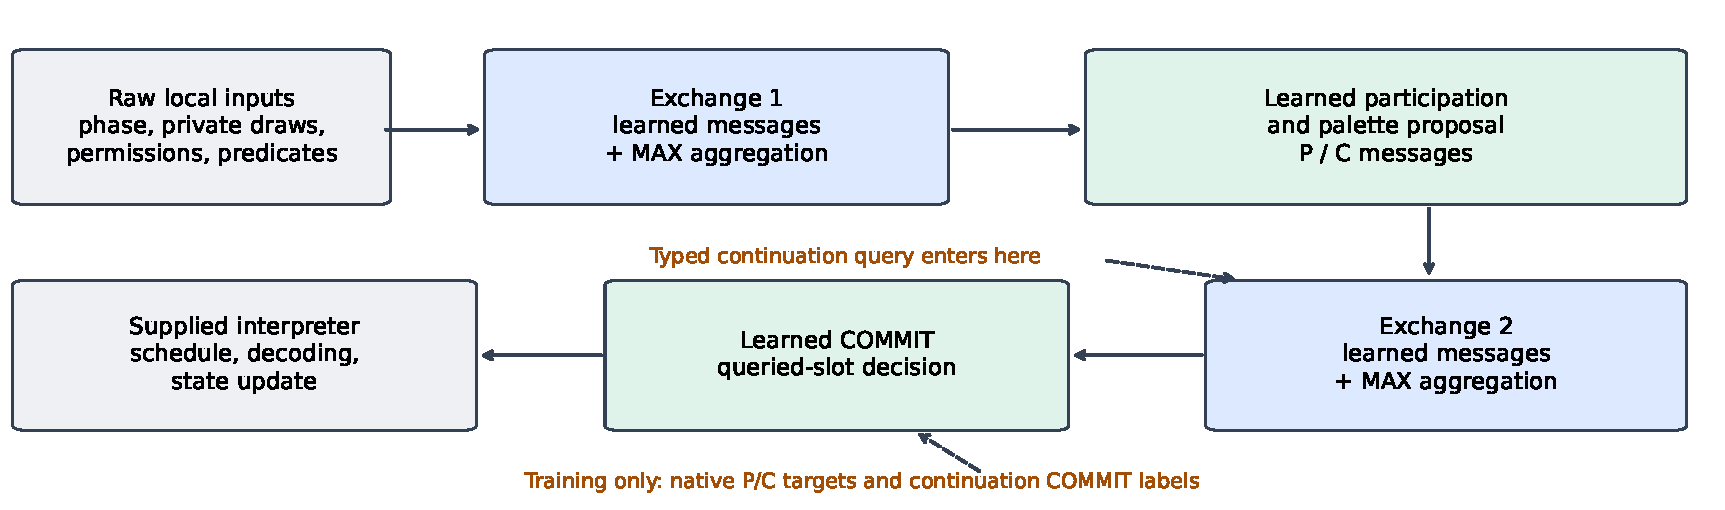
\includegraphics[width=\linewidth]{figures/revision-architecture.pdf}
\caption{Two learned neighbor exchanges inside a supplied state machine.
Each color slot shares parameters; graph messages use MAX. Dashed arrows
locate supplied training targets and diagnostic queries. No continuation oracle or exact
availability filter participates in an autonomous learned rollout.}
\label{fig:architecture}
\end{figure}
The first exchange consumes raw pending/own-color predicates and declared
phase, permission, relative-order or algebraic-equality context. Learned
features feed participation and palette scores. The second exchange consumes
typed P/C messages and raw color predicates, then reads the queried slot's
COMMIT logit. ColorTrials instead exchanges per-color preference/features
and selects its candidate after that exchange. GM DETECT queries the current
color to predict a mark. Hidden-state transformations and message functions
are learned; the interpreter supplies scheduling, list positions, action
decoding, program color/auxiliary updates and phase/queue advancement.
This decomposition locates the continuation query precisely and separates
learned decisions from the externally provided computation.
